\documentclass[CJKutf8,dvipsnames,table]{beamer}
\usepackage{hyperref}
\hypersetup{
  pdfpagemode={FullScreen},
  colorlinks={true},
  linkcolor={blue},
}

%% https://tex.stackexchange.com/questions/47576/combining-ifxetex-and-ifluatex-with-the-logical-or-operation
\usepackage{iftex}
\newif\ifxetexorluatex % a new conditional starts as false
\ifnum 0\ifxetex 1\fi\ifluatex 1\fi>0
   \xetexorluatextrue
\fi
\usepackage{ifplatform}
\ifxetexorluatex
	\usepackage[slantfont,boldfont]{xeCJK}
	\ifwindows
		\setCJKmainfont{SimSun} % Windows默认中文字体:中易宋体
	\else
		\ifmacosx
			\setCJKmainfont{STSong} % MacOS默认中文字体:华文宋体
		\else
			\setCJKmainfont{Noto Serif CJK SC} % Linux默认中文字体:思源宋体(By Adobe & Google)
		\fi	
	\fi
\else
	\usepackage{CJKutf8}
\fi

\usepackage[export]{adjustbox}
\usepackage{mathptmx} %pdfTeX error: pdflatex (file fmex9.pfb): cannot open Type 1 font file for reading
                                                 %https://forum.ubuntu.com.cn/viewtopic.php?t=269943
\usepackage{mathtools}
\usepackage[mathscr]{urwchancal}
\usepackage{amssymb}

\usetheme{Madrid}%{Warsaw}
\usecolortheme{default}

\setbeamertemplate{footline}[page number]{} %gets rid of bottom navigation bars
\setbeamertemplate{navigation symbols}{} %gets rid of navigation symbols

\title{数字信号处理}
\subtitle{第8讲:拉普拉斯变换}
\author{洪明坚}
\institute{重庆大学软件学院}
\date{\today}
  
\begin{document}
\ifxetexorluatex\else
\begin{CJK*}{UTF8}{song}  
\fi

  \AtBeginSection[]
  {
    \begin{frame}
      \frametitle{Outline}
      \tableofcontents[currentsection]
    \end{frame}
  }

  \frame{\titlepage}
  \frame{\frametitle{目录}\tableofcontents}
  
  \section{拉普拉斯变换}
  
  %% PAGE
  \begin{frame}
    \frametitle{回顾:连续时间LTI系统的系统函数}
    \begin{itemize}
    \item 假设$h(t)$是一个LTI系统的单位冲激响应,则该系统对输入$x(t)=e^{st}, s \in \mathbb{C}$的响应
    	\begin{align*}
 		y(t) & = x(t) * h(t) \\
		& = \int_R h(\tau)x(t - \tau )d\tau \\
		& = \int_R h(\tau )e^{s(t-\tau )}d\tau    \\
		& = e^{st} \int_R h(\tau)e^{-s\tau}d\tau \\
		& = H(s)e^{st}
    	\end{align*}   
		\begin{itemize}
		\item 称\[ H(s) = \int_R h(\tau)e^{-s\tau}d\tau \] 为LTI的系统函数(system function)
		\end{itemize}
    \end{itemize}
  \end{frame}  
    
  %% PAGE
  \begin{frame}
    \frametitle{定义}
    \begin{itemize}
    \item 对于一个信号$x(t)$,定义它的拉普拉斯变换(Laplace transform)如下
    \[
	    \mathscr{L}\{x(t)\} = X(s) \triangleq \int_R x(t)e^{-st}dt
    \]
    记为
    \[
    	x(t) \xleftrightarrow{\mathscr{L}} X(s)
    \]
    令$s=\sigma + j\omega$,可以写成
    \begin{align*}
    	X(s) = X(\sigma + j\omega) & = \int_R x(t)e^{-(\sigma + j\omega)t}dt \\
	                        %& = \int_R [x(t)e^{-\sigma t}] e^{-j\omega t}dt \\
	                        & = \mathscr{F}\{ x(t) e^{-\sigma t} \}
    \end{align*}    
    当$\sigma=0$,即$s=j\omega$时,
    \[
    	\left. X(s) \right\vert_{s=j\omega} = \mathscr{F}\{x(t)\}
    \]
    拉普拉斯变换退化为傅立叶变换。
    \item 在傅立叶变换中,频率$\omega$是实数,称为实频域,简称频域;而拉普拉斯变换中频率$s$是复数,一般称为复频域。
    \end{itemize}
  \end{frame}  
      
  %% PAGE
  \begin{frame}
    \frametitle{定义}
    \begin{center}
      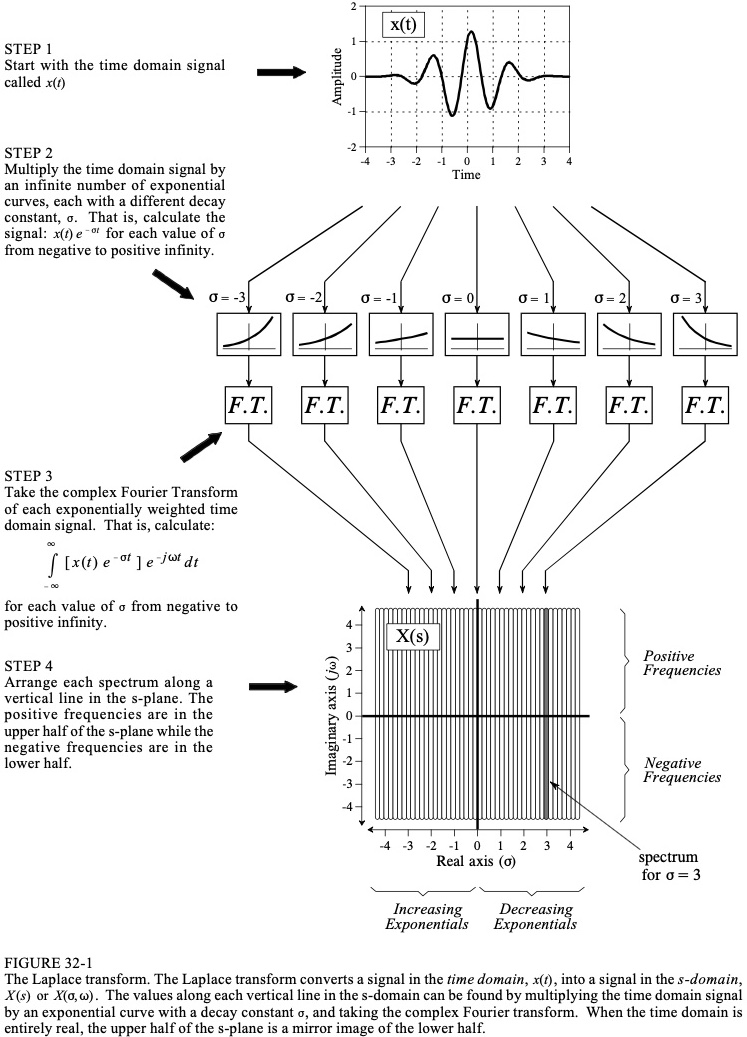
\includegraphics[scale=.227]{segdsp-f32-1}
    \end{center}
  \end{frame}       
      
  %% PAGE
  \begin{frame}
    \frametitle{例子}
    \begin{itemize}
    \item 信号
    \[
    	x(t) = e^{-at}u(t)
    \]
    的傅立叶变换
    \[
    	X(j\omega) = \mathscr{F}\{e^{-at} u(t)\} = \int_{0}^{\infty} e^{-at} e^{-j\omega t} dt = \frac{1}{j\omega + a}, a > 0
    \]
    它的拉普拉斯变换
    \begin{align*}
    	X(s) = X(\sigma + j\omega) = \mathscr{F}\{e^{-(\sigma + a)t} u(t)\} & = \frac{1}{j\omega + (\sigma + a)}, \sigma+a>0 \\
	        & = \frac{1}{s+a}, \operatorname{Re}\{s\} > -a       
    \end{align*}
    \end{itemize}
  \end{frame} 
  
  %% PAGE
  \begin{frame}
    \frametitle{例子}
    \begin{itemize}
    \item 单位冲激函数
    \[
		\mathscr{L}\{\delta(t)\} = \int_R \delta(t)e^{-st} dt = 1
    \]
    \[
    	%https://en.wikipedia.org/wiki/Dirac_delta_function
		\mathscr{L}\{\delta'(t)\} = \int_R \delta'(t)e^{-st} dt = -\left. \frac{d}{dt}e^{-st} \right\vert_{t=0} = s
    \]
    \[
		\mathscr{L}\{\delta^{(k)}(t)\} = \int_R \delta^{(k)}(t)e^{-st} dt = (-1)^k\left. \frac{d^k}{dt^k}e^{-st} \right\vert_{t=0} = s^k
    \]
    \end{itemize}
  \end{frame} 
    
  %% PAGE
  \begin{frame}
    \frametitle{拉普拉斯变换存在与否}
    \begin{itemize}
    \item 不是所有信号都有拉普拉斯变换。前面的例子中,拉普拉斯变换存在的条件是$\operatorname{Re}\{s\} > -a$
		\begin{itemize}
		\item 当$a>0$时,傅立叶变换存在;
		\item 当$a \leq 0$时,傅立叶变换$X(j\omega)$不存在,但拉普拉斯变换$X(s)$存在。
		\end{itemize}
	\item 例子
    	\begin{itemize}
    	\item 信号
    	\[
    		x(t) = -e^{-at}u(-t)
    	\]
    	的拉普拉斯变换
    	\begin{align*}
    		X(s) = -\int_{-\infty}^{\infty} e^{-at} u(-t) e^{-st} dt & = -\int_{-\infty}^{0} e^{-(s+a)t} dt \\
	        	                                                     & = \frac{1}{s+a}       
    	\end{align*}
    	存在的条件是$\operatorname{Re}\{s+a\} < 0$,即$\operatorname{Re}\{s\} < -a$
    	\end{itemize}	
   	\end{itemize}
  \end{frame}  
       
  %% PAGE
  \begin{frame}
    \frametitle{拉普拉斯变换的收敛域}
    \begin{itemize}
    \item 把拉普拉斯变换存在时$s$的取值范围,称为收敛域(Region of convergence, ROC)
	\item 从前面的两个例子可以看出,不同的信号可能具有相同的拉普拉斯变换代数表达式,但它们的ROC却大不相同。
		\begin{itemize}
		\item 因此,在给出一个信号的拉普拉斯变换时,代数表达式和ROC应该同时给出。如 \\
	\begin{tabular}{ll}
	\raisebox{-.5\height}

		$
			e^{-at}u(t) \xleftrightarrow{\mathscr{L}} \frac{1}{s+a}, \operatorname{Re}\{s\} > -a
		$
&
    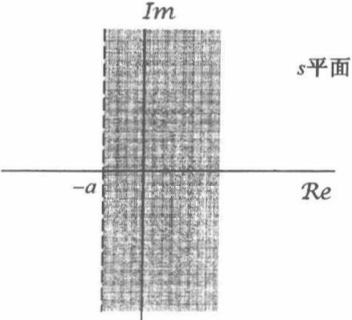
\includegraphics[valign=m,scale=.2]{ss-c-f9-1a}    \\
    \end{tabular} 

		和 \\
	\begin{tabular}{ll}
	\raisebox{-.5\height}

		$
			-e^{-at}u(-t) \xleftrightarrow{\mathscr{L}} \frac{1}{s+a}, \operatorname{Re}\{s\} < -a
		$
&
    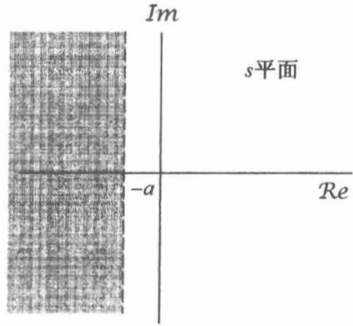
\includegraphics[valign=m,scale=.2]{ss-c-f9-1b}    \\
    \end{tabular}  		

		\end{itemize}
   	\end{itemize}
  \end{frame} 
        
  %% PAGE
  \begin{frame}
    \frametitle{例子}
    \begin{itemize}
    \item 信号
    \[
    	x(t) = e^{-2t}u(t)+e^{-t}cos(3t)u(t) = [e^{-2t}+\frac{1}{2}e^{-(1-3j)t}+\frac{1}{2}e^{-(1+3j)t}]u(t)
    \]
    因为
    \[
    	e^{-2t}u(t) \xleftrightarrow{\mathscr{L}} \frac{1}{s+2}, \operatorname{Re}\{s\}>-2 
    \]
	\[
    	e^{-(1-3j)t}u(t) \xleftrightarrow{\mathscr{L}} \frac{1}{s+(1-3j)}, \operatorname{Re}\{s\}>-1 
    \]
	\[
    	e^{-(1+3j)t}u(t) \xleftrightarrow{\mathscr{L}} \frac{1}{s+(1+3j)}, \operatorname{Re}\{s\}>-1
    \]
    所以
    \begin{align*}
    	X(s) & = \frac{1}{s+2} + \frac{1}{2(s+(1-3j))} + \frac{1}{2(s+(1+3j))} \\
	         & = \frac{2s^2+5s+12}{(s^2+2s+10)(s+2)}, \operatorname{Re}\{s\}>-1
    \end{align*}
    \end{itemize}
  \end{frame}  
         
  %% PAGE
  \begin{frame}
    \frametitle{拉普拉斯变换的零点和极点}
    \begin{itemize}
    \item 上述例子的拉普拉斯变换都是有理的,即可以表示为复变量$s$的两个多项式之比
    \[
    	X(s) = \frac{N(s)}{D(s)}
    \]
    因为多项式可以用它的根来表示,所以
	\[
		X(s) = M\frac{\prod_{i=1}^{R}(s-\beta_i)}{\prod_{j=1}^{P}(s-\alpha_j)}
	\]   
    	\begin{itemize}
    	\item 因为$X(\alpha_j)=\infty$,称$\alpha_j$为极点(pole)
    	\item 因为$X(\beta_i)=0$,称$\beta_i$为零点(zero)
		\item 如果$R > P$,$X(s)$在$\infty$处有一个$(R-P)$阶极点
		\item 如果$R < P$,$X(s)$在$\infty$处有一个$(P-R)$阶零点
    	\end{itemize}	 
    \end{itemize}
  \end{frame}  
  
  %% PAGE
  \begin{frame}
    \frametitle{零点-极点图}
    \begin{itemize}
	\item 用$s$平面上的零点($\bigcirc$)和极点($\times$)来表示$X(s)$,称为$X(s)$的\textbf{零点-极点图(pole-zero plot)}
		\begin{itemize}
		\item 除了一个常数因子外,一个有理拉普拉斯变换可以用零点-极点图和ROC完全表征	
		\end{itemize}
	\item 例子
	\begin{align*}
	   	X(s) & = \frac{1}{s+2} + \frac{1}{2(s+(1-3j))} + \frac{1}{2(s+(1+3j))} = \frac{2s^2+5s+12}{(s^2+2s+10)(s+2)} \\
		     & = \frac{(s+\frac{5+j\sqrt{71}}{4})(s+\frac{5-j\sqrt{71}}{4})}{(s+2)(s+(1-3j))(s+(1+3j))}, \operatorname{Re}\{s\}>-1
	\end{align*}
	的零点-极点图和ROC。注意$X(s)$在$\infty$处有一个零点。
		\begin{center}
    	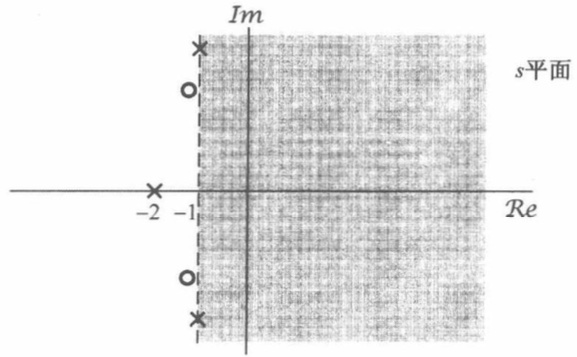
\includegraphics[scale=.28]{ss-c-f9-2b}
    	\end{center}
    \end{itemize}
  \end{frame}  
      
  %% PAGE
  \begin{frame}
    \frametitle{例子}
    \begin{itemize}
	\item 信号
	\[
		x(t) = \delta(t) - \frac{4}{3}e^{-t}u(t)+\frac{1}{3}e^{2t}u(t)
	\]
	因为
	\[
		\mathscr{L}\{\delta(t)\} = \int_R \delta(t)e^{-st} dt = 1
	\]
	所以
	\[
	   	X(s)  = 1 - \frac{4}{3}\frac{1}{s+1} + \frac{1}{3}\frac{1}{s-2} = \frac{(s-1)^2}{(s+1)(s-2)}, \operatorname{Re}\{s\} > 2
	\]
		\begin{center}
    	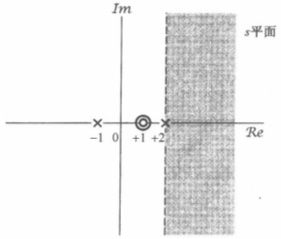
\includegraphics[scale=.47]{ss-c-f9-3}
    	\end{center}
    \end{itemize}
  \end{frame}  
                  
  %% PAGE
  \begin{frame}
    \frametitle{Questions}
    \begin{itemize}
    \item Any questions?
    \end{itemize}
    \begin{center}
      
\includegraphics[scale=.5]{question}
    \end{center}
  \end{frame} 
  
  \section{收敛域的性质} 
  
  %% PAGE
  \begin{frame}
    \frametitle{性质}
    \begin{itemize}
    \item 1、$X(s)$的ROC在$s$平面内由平行于$j\omega$轴的带状区域组成。
    	\begin{itemize}
		\item 因为
    		\begin{align*}
    			X(s) = X(\sigma + j\omega) & = \int_R x(t)e^{-(\sigma + j\omega)t}dt \\
	                                       & = \int_R [x(t)e^{-\sigma t}] e^{-j\omega t}dt \\
	                                       & = \mathscr{F}\{ x(t) e^{-\sigma t} \}
    		\end{align*}
		而$\mathscr{F}\{ x(t) e^{-\sigma t} \}$存在的条件
		\[
			\int_R |x(t)|e^{-\sigma t}dt < \infty
		\]
		只与$\operatorname{Re}\{s\}=\sigma$有关,与$\operatorname{Im}\{s\}=\omega$无关。
		\end{itemize}
    \end{itemize}
  \end{frame} 
    
  %% PAGE
  \begin{frame}
    \frametitle{性质}
    \begin{itemize}
    \item 2、对有理拉普拉斯变换来说,ROC内不包含任何极点。
    \item 3、如果$x(t)$是有限持续期,且是绝对可积的,那么它的ROC是整个$s$平面
    	\begin{itemize}
		\item 因为
    		\[
    			\int_{T_1}^{T_2} |x(t)| dt < \infty \Rightarrow \{\operatorname{Re}\{s\}=\sigma = 0\} \subset ROC
    		\]
		以及
		\begin{align*}
			\int_{T_1}^{T_2} |x(t)|e^{-\sigma t}dt & < e^{-\sigma T_1}\int_{T_1}^{T_2} |x(t)| dt \Rightarrow \{\operatorname{Re}\{s\}=\sigma > 0\} \subset ROC \\
			\int_{T_1}^{T_2} |x(t)|e^{-\sigma t}dt & < e^{-\sigma T_2}\int_{T_1}^{T_2} |x(t)| dt \Rightarrow \{\operatorname{Re}\{s\}=\sigma < 0\} \subset ROC
		\end{align*}
		所以,ROC是整个$s$平面。
		
		\item 已知
	\begin{tabular}{ll}
	\raisebox{-.5\height}

    \begin{math}
x(t) = 
\left\{
    \begin {aligned}
         & e^{-at} \quad & 0 < t < T \\
         & 0 \quad & otherwise                 
    \end{aligned}
\right.
	\end{math}
&
     $\xleftrightarrow{\mathscr{L}} \frac{1}{s+a}[1-e^{-(s+a)T}]$ 
    \end{tabular}
     ,问:$s=-a$是不是极点?
		\end{itemize}
    \end{itemize}
  \end{frame} 
      
  %% PAGE
  \begin{frame}
    \frametitle{性质}
    \begin{itemize}
    \item 4、如果$x(t)$是右边(right-sided)信号,且$\operatorname{Re}\{s\}=\sigma_0$这条线位于ROC内,那么$\operatorname{Re}\{s\}>\sigma_0$的全部$s$值一定在ROC内。   
		\begin{tabular}{ll}
		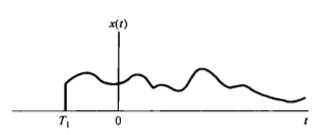
\includegraphics[scale=.45]{ss-c-f9-6}
		&
     	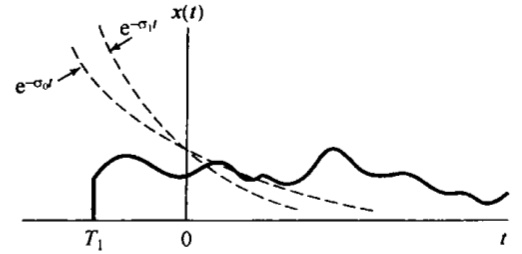
\includegraphics[scale=.3]{ss-c-f9-7}
    	\end{tabular} 
    	\[  
     	\int_{T_1}^{\infty} |x(t)|e^{-\sigma_1 t}dt  < \int_{T_1}^{\infty} |x(t)| e^{-\sigma_0 T_1} dt, \sigma_1 > \sigma_0
    	\]
    \item 5、如果$x(t)$是左边(left-sided)信号,且$\operatorname{Re}\{s\}=\sigma_0$这条线位于ROC内,那么$\operatorname{Re}\{s\}<\sigma_0$的全部$s$值一定在ROC内。   
    \end{itemize}
  \end{frame} 

  %% PAGE
  \begin{frame}
    \frametitle{性质}
    \begin{itemize}
    \item 6、如果$x(t)$是双边(two-sided)信号,且$\operatorname{Re}\{s\}=\sigma_0$这条线位于ROC内,那么ROC一定由$s$平面的一条带状区域组成,且直线$\operatorname{Re}\{s\}=\sigma_0$位于带中。   
    \begin{itemize}
    \item 例子
    \[
    	x(t) = e^{-b|t|}=e^{-bt}u(t)+e^{bt}u(-t)
    \]
    \[
    	e^{-bt}u(t) \xleftrightarrow{\mathscr{L}} \frac{1}{s+b}, \operatorname{Re}\{s\} > -b
    \]
    \[
    	e^{bt}u(-t) \xleftrightarrow{\mathscr{L}} \frac{-1}{s-b}, \operatorname{Re}\{s\} < b
    \]
    尽管两个单独项都有拉普拉斯变换,但是当$b \leq 0$时,$x(t)$没有拉普拉斯变换。当$b>0$时,有
    \[
    	e^{-b|t|} \xleftrightarrow{\mathscr{L}} \frac{1}{s+b} - \frac{1}{s-b}=\frac{-2b}{(s-b)(s+b)}, -b < \operatorname{Re}\{s\} < b
    \]
    
    \end{itemize}
		\begin{center}
		\begin{tabular}{ll}
		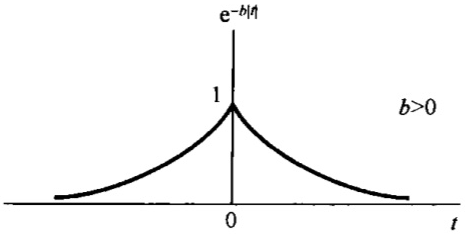
\includegraphics[scale=.2]{ss-c-f9-11a}
		&
		%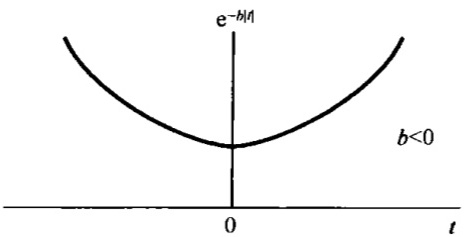
\includegraphics[scale=.23]{ss-c-f9-11b}
		%&
     	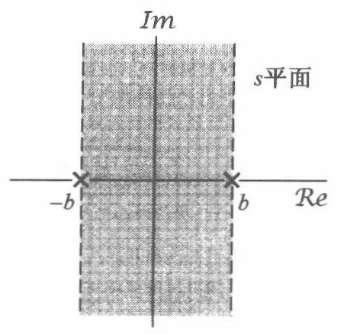
\includegraphics[scale=.2]{ss-c-f9-12}
    	\end{tabular} 
		\end{center}
    \end{itemize}
  \end{frame}      
         
  %% PAGE
  \begin{frame}
    \frametitle{性质}
    \begin{itemize}
    \item 7、如果$x(t)$的拉普拉斯变换$X(s)$是有理的,那么ROC是被极点所界定的或延伸到$\infty$,而且在ROC内不包含任何极点。   
    \item 8、如果$x(t)$的拉普拉斯变换$X(s)$是有理的,那么
    	\begin{itemize}
    	\item 若$x(t)$是右边信号,则ROC在s平面位于最右边极点的右边;
    	\item 若$x(t)$是左边信号,则ROC在s平面位于最左边极点的左边。
    	\end{itemize}
	\item 例子
		\begin{itemize}
		\item 某一拉普拉斯变换的代数表达式为
		\[
			X(s) = \frac{1}{(s+1)(s+2)}
		\]
		它的极点分布,以及三种可能的ROC
		\end{itemize}
		\begin{center}
    	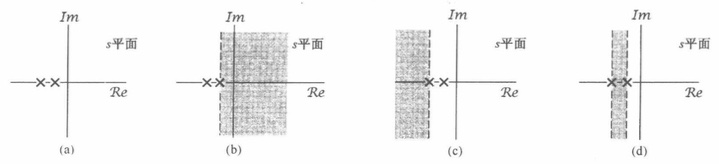
\includegraphics[scale=.42]{ss-c-f9-13}
    	\end{center}
    \end{itemize}
  \end{frame}
         
  %% PAGE
  \begin{frame}
    \frametitle{Questions}
    \begin{itemize}
    \item Any questions?
    \end{itemize}
    \begin{center}
      
\includegraphics[scale=.5]{question}
    \end{center}
  \end{frame} 
  
  \section{拉普拉斯逆变换}
  
  %% PAGE
  \begin{frame}
    \frametitle{拉普拉斯逆变换}
    \begin{itemize}
    \item 根据拉普拉斯变换的定义
	\[
    	X(s) = X(\sigma + j\omega) = \mathscr{F}\{ x(t) e^{-\sigma t} \}
	         = \int_R x(t)e^{-(\sigma + j\omega)t}dt 
	\]
	\item 利用傅立叶逆变换
	\[
    	x(t) e^{-\sigma t} = \mathscr{F}^{-1}\{ X(\sigma + j\omega) \}   
	                       = \frac{1}{2\pi}\int_R X(\sigma + j\omega)e^{j\omega t}d\omega 
	\]
	两边同乘以$e^{\sigma t}$得到
	\[
		x(t) = \frac{1}{2\pi}\int_R X(\sigma + j\omega)e^{(\sigma+j\omega) t}d\omega 
	\]
	因为$s=\sigma+j\omega$,固定$\sigma$,有$ds=jd\omega$
	\[
		x(t) = \frac{1}{2\pi j}\int_{\sigma-j\omega}^{\sigma+j\omega} X(s)e^{st}ds 	
	\]
	该式对于任意一条在ROC中的直线$\operatorname{Re}\{s\}=\sigma$都成立。
    \end{itemize}
  \end{frame}   

  %% PAGE
  \begin{frame}
    \frametitle{拉普拉斯逆变换}
    \begin{itemize}
    \item 用定义直接求拉普拉斯逆变换涉及到复变函数中用留数定理求解围线积分(contour integration),比较麻烦。对于有理变换,有更加简便的方法。
	\item 有理拉普拉斯变换可以展开成部分分式之和
	\[
		X(s) = \sum_{i=1}^{r} \sum_{k_i=1}^{N_i} \frac{A_{i,k_i}}{(s+a_i)^{k_i}}
	\]
	利用已知的变换对
	\begin{align*}
		\frac{t^{n-1}}{(n-1)!}e^{-at}u(t) & \xleftrightarrow{\mathscr{L}} \frac{1}{(s+a)^n}, \operatorname{Re}\{s\} > -a \\
		-\frac{t^{n-1}}{(n-1)!}e^{-at}u(-t) & \xleftrightarrow{\mathscr{L}} \frac{1}{(s+a)^n}, \operatorname{Re}\{s\} < -a
	\end{align*}
    \end{itemize}
  \end{frame}   
    
  %% PAGE
  \begin{frame}
    \frametitle{例子}
    \begin{itemize}
    \item 考虑如下拉普拉斯变换
	\[
	   	X(s)  = \frac{1}{(s+1)(s+2)^2} = \frac{1}{s+1} - \frac{1}{s+2} - \frac{1}{(s+2)^2}
	\]
	有两个极点$s=-1$和$s=-2$。
		\begin{itemize}
		\item 1、如果ROC是$\operatorname{Re}\{s\} > -1$,因为
		\begin{align*}
			e^{-t}u(t) & \xleftrightarrow{\mathscr{L}} \frac{1}{s+1}, \operatorname{Re}\{s\} > -1 \\
			e^{-2t}u(t) & \xleftrightarrow{\mathscr{L}} \frac{1}{s+2}, \operatorname{Re}\{s\} > -2 \\
			te^{-2t}u(t) & \xleftrightarrow{\mathscr{L}} \frac{1}{(s+2)^2}, \operatorname{Re}\{s\} > -2 
		\end{align*}
		所以
		\[
			x(t) = e^{-t}u(t) - e^{-2t}u(t) - te^{-2t}u(t)
		\]
		\end{itemize}
    \end{itemize}
  \end{frame}  
      
  %% PAGE
  \begin{frame}
    \frametitle{例子}
    \begin{itemize}
    \item 考虑如下拉普拉斯变换
	\[
	   	X(s)  = \frac{1}{(s+1)(s+2)^2} = \frac{1}{s+1} - \frac{1}{s+2} - \frac{1}{(s+2)^2}
	\]
	有两个极点$s=-1$和$s=-2$。
		\begin{itemize}
		\item 2、如果ROC是$\operatorname{Re}\{s\} < -2$,因为
		\begin{align*}
			-e^{-t}u(-t) & \xleftrightarrow{\mathscr{L}} \frac{1}{s+1}, \operatorname{Re}\{s\} < -1 \\
			-e^{-2t}u(-t) & \xleftrightarrow{\mathscr{L}} \frac{1}{s+2}, \operatorname{Re}\{s\} < -2 \\
			-te^{-2t}u(-t) & \xleftrightarrow{\mathscr{L}} \frac{1}{(s+2)^2}, \operatorname{Re}\{s\} < -2 
		\end{align*}
		所以
		\[
			x(t) = -e^{-t}u(-t) + e^{-2t}u(-t) + te^{-2t}u(-t)
		\]
		\end{itemize}
    \end{itemize}
  \end{frame}  
        
  %% PAGE
  \begin{frame}
    \frametitle{例子}
    \begin{itemize}
    \item 考虑如下拉普拉斯变换
	\[
	   	X(s)  = \frac{1}{(s+1)(s+2)^2} = \frac{1}{s+1} - \frac{1}{s+2} - \frac{1}{(s+2)^2}
	\]
	有两个极点$s=-1$和$s=-2$。
		\begin{itemize}
		\item 3、如果ROC是$-2 < \operatorname{Re}\{s\} < -1$,因为
		\begin{align*}
			-e^{-t}u(-t) & \xleftrightarrow{\mathscr{L}} \frac{1}{s+1}, \operatorname{Re}\{s\} < -1 \\
			e^{-2t}u(t) & \xleftrightarrow{\mathscr{L}} \frac{1}{s+2}, \operatorname{Re}\{s\} > -2 \\
			te^{-2t}u(t) & \xleftrightarrow{\mathscr{L}} \frac{1}{(s+2)^2}, \operatorname{Re}\{s\} > -2 
		\end{align*}
		所以
		\[
			x(t) = -e^{-t}u(-t) - e^{-2t}u(t) - te^{-2t}u(t)
		\]
		\end{itemize}
    \end{itemize}
  \end{frame}  
    
  %% PAGE
  \begin{frame}
    \frametitle{基本函数的拉普拉斯变换}
    \begin{center}
      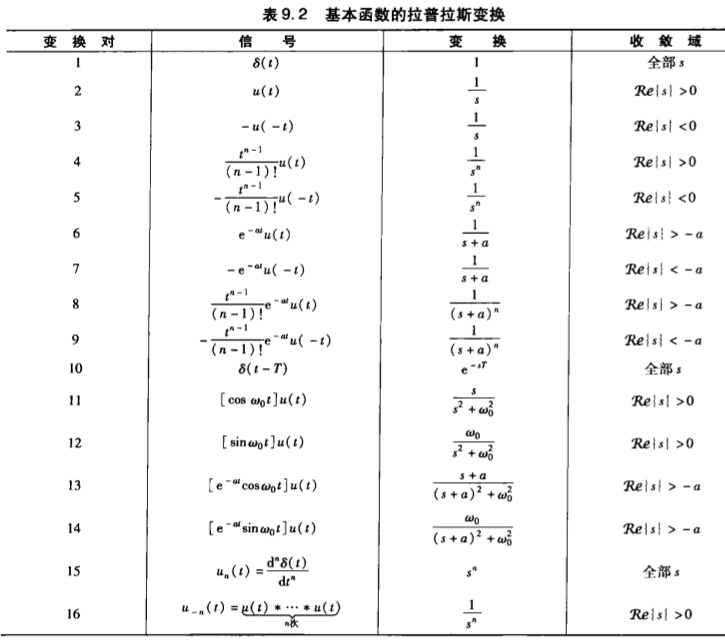
\includegraphics[scale=.37]{ss-c-t9-2}
    \end{center}
  \end{frame}   
            
  %% PAGE
  \begin{frame}
    \frametitle{Questions}
    \begin{itemize}
    \item Any questions?
    \end{itemize}
    \begin{center}
      
\includegraphics[scale=.5]{question}
    \end{center}
  \end{frame}
  
  \section{用零极图分析频率响应特性}
  
  %% PAGE
  \begin{frame}
    \frametitle{零点向量和极点向量}
    \begin{itemize}
	\item 如果
	\[
	X(s)=s-a
	\]
	则$a$是一个零点,对于$s$平面中任意一点$s_1$,称$s_1-a$为零点向量
		\begin{itemize}
		\item $X(s_1)$的模就是向量的长度,相位就是该向量与实轴$\operatorname{Re}$的夹角
		\end{itemize}
	\item 如果
	\[
	X(s)=\frac{1}{s-a}
	\]
	则$a$是一个极点,对于$s$平面中任意一点$s_1$,称$s_1-a$为极点向量
		\begin{itemize}
		\item $X(s_1)$的模就是向量的长度的倒数,相位就是该向量与实轴$\operatorname{Re}$的夹角的负值
		\end{itemize}

    \end{itemize}
    \begin{center}
      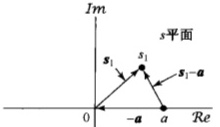
\includegraphics[scale=.5]{ss-c-f9-15}
    \end{center}
  \end{frame}
  
  %% PAGE
  \begin{frame}
    \frametitle{用零极图分析频率响应特性}
    \begin{itemize}
    \item 对于一般的有理拉普拉斯变换
	\[
		X(s) = M\frac{\prod_{i=1}^{R}(s-\beta_i)}{\prod_{j=1}^{P}(s-\alpha_j)}
	\]
	$X(s_1)$的模就是各零点向量长度之积的M倍除以各极点向量长度之积,相位就是零点相位之和减去极点的相位之和
    \end{itemize}
  \end{frame}    
  
  %% PAGE
  \begin{frame}
    \frametitle{用零极图分析频率响应特性}
    \begin{itemize}
    \item 例子1   
\[
X(s)=\frac{1}{s+1/\tau}, \operatorname{Re}\{s\} > -1/\tau
\]
它的傅立叶变换
\[
X(j\omega)=\frac{1}{j\omega+1/\tau}
\]
它的零点-极点图($\tau=2$)
    \begin{center}
      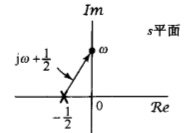
\includegraphics[scale=.5]{ss-c-f9-16}
    \end{center}
    和频率及相位响应曲线
    \begin{center}
      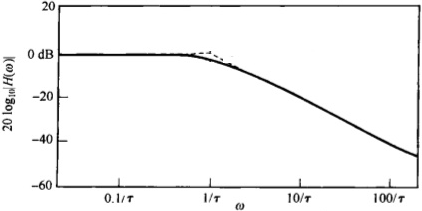
\includegraphics[scale=.27]{ss-c-f9-18a}
      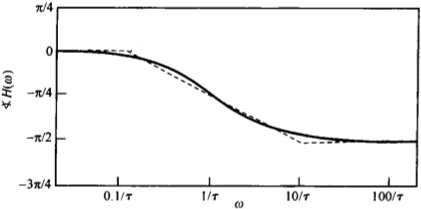
\includegraphics[scale=.27]{ss-c-f9-18b}
    \end{center}

    \end{itemize}
     
  \end{frame}     
  
  %% PAGE
  \begin{frame}
    \frametitle{用零极图分析频率响应特性}
    \begin{itemize}
    \item 例子2   
\[
X(s)=\frac{s-a}{s+a}, \operatorname{Re}\{s\} > -a
\]
它的零点-极点图和频率及相位响应曲线
    \begin{center}
      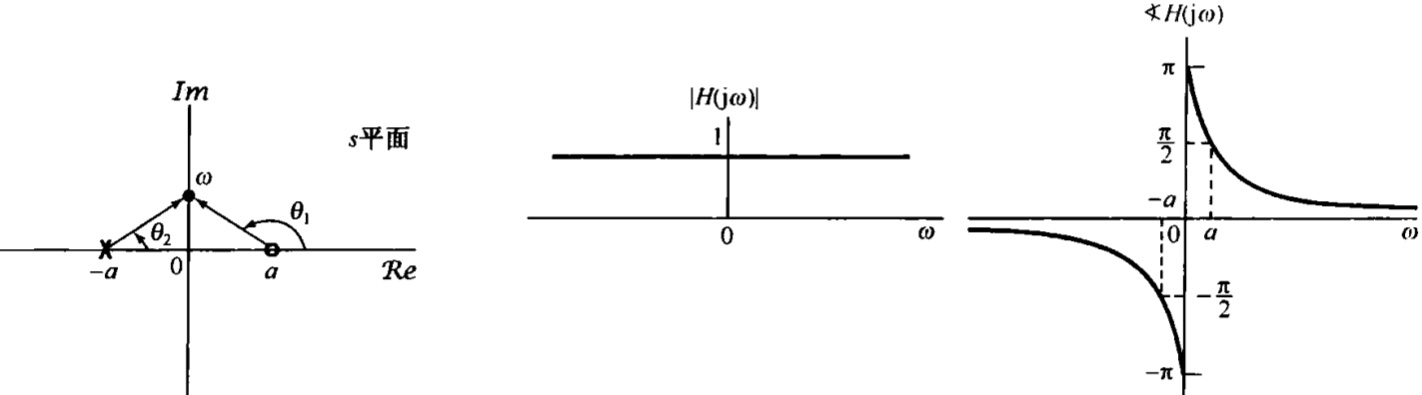
\includegraphics[scale=.22]{ss-c-f9-21}
    \end{center}
    	\begin{itemize}
    	\item 
    	\[
    	|H(j\omega)| = 1
    	\]
    	\[    
    	arg\{ H(j\omega) \}= \theta_1 - \theta_2 = \pi - 2\theta_2 = \pi - 2arctan(\frac{\omega}{a})
    	\]
    	\end{itemize}
	这是一个全通系统(all-pass system)。
    \end{itemize}     
  \end{frame}     
    
  %% PAGE
  \begin{frame}
    \frametitle{Questions}
    \begin{itemize}
    \item Any questions?
    \end{itemize}
    \begin{center}
      
\includegraphics[scale=.5]{question}
    \end{center}
  \end{frame}  
  
  \section{拉普拉斯变换的性质}
  
  %% PAGE
  \begin{frame}
    \frametitle{性质}
    \begin{itemize}
    \item 1、线性
    若
    \[
    x_1(t) \xleftrightarrow{\mathscr{L}} X_1(s), ROC=R_1
    \]
    \[
    x_2(t) \xleftrightarrow{\mathscr{L}} X_2(s), ROC=R_2
    \]
    则
    \[
    ax_1(t)+bx_2(t) \xleftrightarrow{\mathscr{L}} aX_1(s)+bX_2(s), R_1 \cap R_2 \subset ROC 
    \]
    	\begin{itemize}
    	\item 如果$R_1 \cap R_2=\emptyset$,则拉普拉斯变换不存在。
   		\item 注意:ROC可能比$R_1 \cap R_2$大。
			\begin{itemize}
			\item 如果$x_1(t)=x_2(t)$,且$a=-b$,则$x(t)=0$,因此$X(s)=0$,ROC是整个s平面。
			\end{itemize}
    	\end{itemize}
    \end{itemize}
  \end{frame} 
    
  %% PAGE
  \begin{frame}
    \frametitle{性质}
    \begin{itemize}
    \item 2、时域平移 \\
    \[
    x(t-t_0) \xleftrightarrow{\mathscr{L}} e^{-st_0}X(s), ROC=R
    \]
    \item 3、$s$域平移 
    \[
    e^{s_0 t}x(t) \xleftrightarrow{\mathscr{L}} X(s-s_0), ROC=R+\operatorname{Re}\{s_0\}
    \]
    \begin{center}
      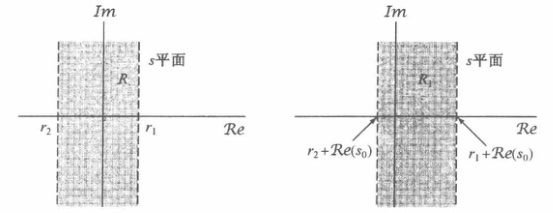
\includegraphics[scale=.5]{ss-c-f9-23}
    \end{center}
    \end{itemize}
  \end{frame}
      
  %% PAGE
  \begin{frame}
    \frametitle{性质}
    \begin{itemize}
    \item 4、卷积 \\
    \[
    x_1(t) \ast x_2(t) \xleftrightarrow{\mathscr{L}} X_1(s)X_2(s), R_1 \cap R_2 \subset ROC 
    \]
    	\begin{itemize}
   		\item 注意:ROC可能比$R_1 \cap R_2$大。
			\begin{itemize}
			\item 如果
			\[
			X_1(s)=\frac{s+1}{s+2}, \operatorname{Re}\{s\} > -2
			\]
			\[
			X_1(s)=\frac{s+2}{s+1}, \operatorname{Re}\{s\} > -1
			\]
			则$X_1(s)X_2(s)=1$,ROC是整个s平面。
			\end{itemize}
    	\end{itemize}
    \end{itemize}
  \end{frame}
   
  %% PAGE
  \begin{frame}
    \frametitle{性质}
    \begin{itemize}
    \item 5、时域微分 \\
    \[
    \frac{dx(t)}{dt} \xleftrightarrow{\mathscr{L}} sX(s), R \subset ROC 
    \]
    	\begin{itemize}
		\item 方法1:对下式求$t$的导数
		\[
				x(t) = \frac{1}{2\pi j}\int_{\sigma-j\omega}^{\sigma+j\omega} X(s)e^{st}ds 	
		\]
		可得
		\[
				\frac{d}{dt}x(t) = \frac{1}{2\pi j}\int_{\sigma-j\omega}^{\sigma+j\omega} [sX(s)]e^{st}ds 	
		\]
		\item 方法2:利用卷积性质和$\delta(t)$的性质
		\[
			x'(t) = x(t) \ast \delta'(t) %https://math.stackexchange.com/questions/1912108/convolution-between-the-derivative-dirac-delta-function-and-other-function
		\]
		有
		\[
		\mathscr{L}\{x'(t)\} = \mathscr{L}\{x(t) \ast \delta'(t) \} = \mathscr{L}\{x(t)\} \mathscr{L}\{\delta'(t)\} = \mathscr{L}\{x(t)\}s = sX(s)
		\]
		\end{itemize}
    \end{itemize}
  \end{frame}

  %% PAGE
  \begin{frame}
    \frametitle{性质}
    \begin{itemize}
    \item 6、$s$域微分
    \[
    -tx(t) \xleftrightarrow{\mathscr{L}} \frac{dX(s)}{ds}, ROC=R
    \]
    	\begin{itemize}
    	\item 例子
    	\[
    		e^{-at}u(t) \xleftrightarrow{\mathscr{L}} \frac{1}{s+a}, \operatorname{Re}\{s\} > -a     
    	\]
		利用微分性质
		\[
			te^{-at}u(t) \xleftrightarrow{\mathscr{L}} -\frac{d}{ds}[\frac{1}{s+a}]=\frac{1}{(s+a)^2}, \operatorname{Re}\{s\} > -a 
		\]
		重复利用可得
		\[
			\frac{t^{n-1}}{(n-1)!}e^{-at}u(t) \xleftrightarrow{\mathscr{L}} \frac{1}{(s+a)^n}, \operatorname{Re}\{s\} > -a 		
		\]    
    \end{itemize}
    \end{itemize}
  \end{frame}

  %% PAGE
  \begin{frame}
    \frametitle{性质汇总}
    \begin{center}
      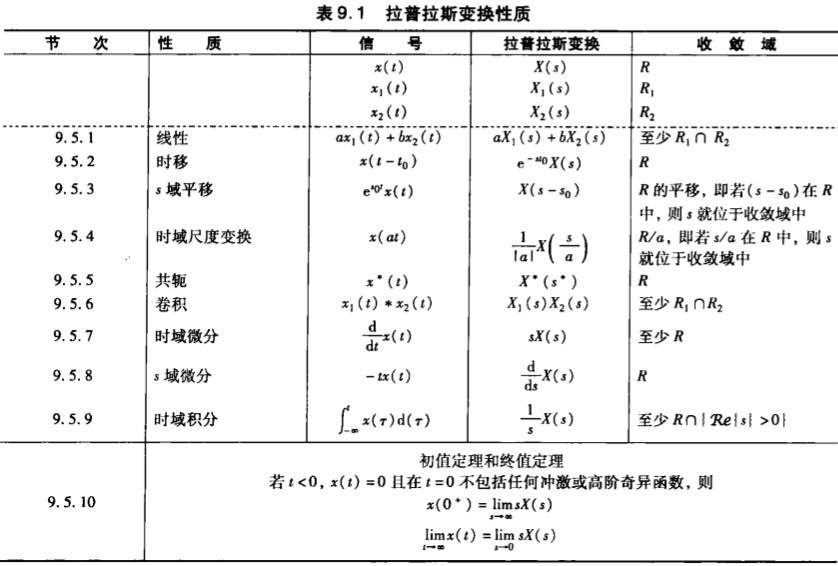
\includegraphics[scale=.4]{ss-c-t9-1}
    \end{center}
  \end{frame}              
          
  %% PAGE
  \begin{frame}
    \frametitle{Questions}
    \begin{itemize}
    \item Any questions?
    \end{itemize}
    \begin{center}
      
\includegraphics[scale=.5]{question}
    \end{center}
  \end{frame}   
  
  \section{用拉普拉斯变换分析LTI系统}
  
  %% PAGE
  \begin{frame}
    \frametitle{LTI系统函数}
    \begin{itemize}
    \item 如果$h(t)$是LTI系统的冲激响应
    \[
    	y(t) = x(t) \ast h(t)
    \]
    根据拉普拉斯变换的卷积性质
    \[
    	Y(s) = X(s)H(s)
    \]
	称
	\[
	H(s) = \int_R h(t)e^{-st}dt
	\]
	为系统函数或转移函数(transfer function)
    \end{itemize}
  \end{frame}   
  
  %% PAGE
  \begin{frame}
    \frametitle{因果性}
    \begin{itemize}
    \item 对于因果的LTI系统,有$h(t)=0, t < 0$,
	%\[
	%	H(s) = \int_R h(t)e^{-st}dt = \int_{0}^{\infty} h(t) e^{-(\sigma+j\omega)t}dt = \int_{0}^{\infty} h(t) e^{-\sigma t} e^{-j\omega t}dt
	%\]
	则它的ROC是某个右半平面
		\begin{itemize}
		\item 例子
		\[
			h(t) = e^{-t}u(t) \xleftrightarrow{\mathscr{L}} H(s) = \frac{1}{s+1}, \operatorname{Re}\{s\} > -1
		\]
		\end{itemize}
	\item 反过来却不成立
		\begin{itemize}
		\item 例子
		\[
			h(t) = e^{-(t+1)}u(t+1) \xleftrightarrow{\mathscr{L}} H(s) = \frac{e^s}{s+1}, \operatorname{Re}\{s\} > -1
		\]
		$h(t) \neq 0, -1 < t < 0$,所以它不是因果的。
		\end{itemize}
	
    \end{itemize}
  \end{frame}   
    
  %% PAGE
  \begin{frame}
    \frametitle{稳定性}
    \begin{itemize}
    \item 对于稳定的LTI系统,有
    \[
    	\int_R |h(t)|dt < \infty
    \]
    此时,单位冲激响应的傅立叶变换(即频率响应)$H(j\omega)$存在。所以,
    \item 当且仅当系统函数$H(s)$的ROC包含$s$平面的虚轴$j\omega$,即$\operatorname{Re}\{s\}=0$时,LTI系统是稳定的。
	\item 综合起来:一个因果的LTI系统是稳定的,当且仅当$H(s)$最右边的极点必须位于$j\omega$轴的左边,即所有极点的实部必须是负数。
	
    \end{itemize}
  \end{frame}   
      
  %% PAGE
  \begin{frame}
    \frametitle{由线性常系数微分方程表征的LTI系统}
    \begin{itemize}
    \item 一个连续时间LTI系统可以用线性常系数微分方程表示
    \[
    	\sum_{k=0}^{N} a_k \frac{d^k y(t)}{dt^k} = \sum_{k=0}^{M} b_k \frac{d^k x(t)}{dt^k}
    \]
    两边进行拉普拉斯变换,反复应用线性和微分性质,可得
    \[
    	(\sum_{k=0}^{N} a_k s^k)Y(s)  = (\sum_{k=0}^{M} b_k s^k ) X(s)
    \]
    因此
    \[
    	H(s) = \frac{Y(s)}{X(s)} = \frac{\sum_{k=0}^{M} b_k s^k}{\sum_{k=0}^{N} a_k s^k}    
    \]
    即,一个由线性常系数微分方程表征的LTI系统,且系统函数总是有理的。
    \item 通过拉普拉斯变换,可以把微分方程转换为代数方程进行求解。
    \end{itemize}
  \end{frame}    
  
  %% PAGE
  \begin{frame}
    \frametitle{例子}
    \begin{itemize}
    \item 对于系统
    \[
    	\frac{dy(t)}{dt} + 3y(t) = x(t)
    \]
    求它的冲激响应。
    \item 两边进行拉普拉斯变换,应用线性和微分性质,可得
    \[
    	sY(s) + 3Y(s) = X(s)
    \]
    因此
    \[
    	H(s) = \frac{Y(s)}{X(s)} = \frac{1}{s+3}    
    \]
    	\begin{itemize}
		\item 如果ROC是$\operatorname{Re}\{s\} > -3$,则$h(t) = e^{-3t}u(t)$
		\item 如果ROC是$\operatorname{Re}\{s\} < -3$,则$h(t) = -e^{-3t}u(-t)$	
		\end{itemize}
		
	\item 可以证明:对于一个有理的LTI系统,系统是因果的等价于ROC位于最右边极点的右边。
    \end{itemize}
  \end{frame}
    
            
  %% PAGE
  \begin{frame}
    \frametitle{Questions}
    \begin{itemize}
    \item Any questions?
    \end{itemize}
    \begin{center}
      
\includegraphics[scale=.5]{question}
    \end{center}
  \end{frame}    
  
\ifxetexorluatex\else
\end{CJK*}  
\fi  
\end{document}

%%% Local Variables: 
%%% mode: latex
%%% TeX-master: t
%%% End: 
